\documentclass[
11pt, % The default document font size, options: 10pt, 11pt, 12pt
codirector, % Uncomment to add a codirector to the title page
]{charter} 




% El títulos de la memoria, se usa en la carátula y se puede usar el cualquier lugar del documento con el comando \ttitle
\titulo{Desarrollo de plataforma móvil para SLAM monocular} 

% Nombre del posgrado, se usa en la carátula y se puede usar el cualquier lugar del documento con el comando \degreename
\posgrado{Carrera de Especialización en Sistemas Embebidos} 
%\posgrado{Carrera de Especialización en Internet de las Cosas} 
%\posgrado{Carrera de Especialización en Intelegencia Artificial}
%\posgrado{Maestría en Sistemas Embebidos} 
%\posgrado{Maestría en Internet de las cosas}

% Tu nombre, se puede usar el cualquier lugar del documento con el comando \authorname
\autor{Ing. Gonzalo Gabriel Fernández} 

% El nombre del director y co-director, se puede usar el cualquier lugar del documento con el comando \supname y \cosupname y \pertesupname y \pertecosupname
\director{Nombre del Director}
\pertenenciaDirector{pertenencia} 
% FIXME:NO IMPLEMENTADO EL CODIRECTOR ni su pertenencia
\codirector{John Doe} % para que aparezca en la portada se debe descomentar la opción codirector en el documentclass
\pertenenciaCoDirector{FIUBA}

% Nombre del cliente, quien va a aprobar los resultados del proyecto, se puede usar con el comando \clientename y \empclientename
\cliente{Ing. Leandro Borgnino}
\empresaCliente{Fundación Fulgor}

% Nombre y pertenencia de los jurados, se pueden usar el cualquier lugar del documento con el comando \jurunoname, \jurdosname y \jurtresname y \perteunoname, \pertedosname y \pertetresname.
\juradoUno{Nombre y Apellido (1)}
\pertenenciaJurUno{pertenencia (1)} 
\juradoDos{Nombre y Apellido (2)}
\pertenenciaJurDos{pertenencia (2)}
\juradoTres{Nombre y Apellido (3)}
\pertenenciaJurTres{pertenencia (3)}
 
\fechaINICIO{25 de abril de 2023}		%Fecha de inicio de la cursada de GdP \fechaInicioName
\fechaFINALPlan{13 de junio de 2023} 	%Fecha de final de cursada de GdP
\fechaFINALTrabajo{15 de mayo de 2024}	%Fecha de defensa pública del trabajo final


\begin{document}

\maketitle
\thispagestyle{empty}
\pagebreak


\thispagestyle{empty}
{\setlength{\parskip}{0pt}
\setcounter{tocdepth}{1}
\tableofcontents{}
}
\pagebreak


\section*{Registros de cambios}
\label{sec:registro}


\begin{table}[ht]
\label{tab:registro}
\centering
\begin{tabularx}{\linewidth}{@{}|c|X|c|@{}}
\hline
\rowcolor[HTML]{C0C0C0} 
Revisión & \multicolumn{1}{c|}{\cellcolor[HTML]{C0C0C0}Detalles de los cambios realizados} & Fecha      \\ \hline
0      & Creación del documento                                 &\fechaInicioName \\ \hline
1      & Se completa hasta el punto 4 inclusive                 & 9 de mayo de 2023 \\ \hline
2      & Se completa hasta el punto 7 inclusive					& 16 de mayo de 2023 \\ \hline
3      & Se completa hasta el punto 12 inclusive                & 25 de mayo de 2023 \\ \hline
%4      & Se completa el plan	                                 & dd/mm/aaaa \\ \hline
\end{tabularx}
\end{table}

\pagebreak



\section*{Acta de constitución del proyecto}
\label{sec:acta}

\begin{flushright}
Córdoba, \fechaInicioName
\end{flushright}

\vspace{2cm}

Por medio de la presente se acuerda con el \authorname\hspace{1px} que su Trabajo Final de la \degreename\hspace{1px} se titulará ``\ttitle'', consistirá esencialmente en el desarrollo de una plataforma móvil para la evaluación de algoritmos de SLAM monocular investigados para aplicación en navegación autónoma, y tendrá un presupuesto preliminar estimado de 600 h de trabajo, con fecha de inicio el \fechaInicioName\hspace{1px} y fecha de presentación pública el \fechaFinalName.

Se adjunta a esta acta la planificación inicial.

\vfill

% Esta parte se construye sola con la información que hayan cargado en el preámbulo del documento y no debe modificarla
\begin{table}[ht]
\centering
\begin{tabular}{ccc}
\begin{tabular}[c]{@{}c@{}}Dr. Ing. Ariel Lutenberg \\ Director posgrado FIUBA\end{tabular} & \hspace{2cm} & \begin{tabular}[c]{@{}c@{}}\clientename \\ \empclientename \end{tabular} \vspace{2.5cm} \\ 
\multicolumn{3}{c}{\begin{tabular}[c]{@{}c@{}} \supname \\ Director del Trabajo Final\end{tabular}} \vspace{2.5cm} \\
%\begin{tabular}[c]{@{}c@{}}\jurunoname \\ Jurado del Trabajo Final\end{tabular}     &  & \begin{tabular}[c]{@{}c@{}}\jurdosname\\ Jurado del Trabajo Final\end{tabular}  \vspace{2.5cm}  \\
%\multicolumn{3}{c}{\begin{tabular}[c]{@{}c@{}} \jurtresname\\ Jurado del Trabajo Final\end{tabular}} \vspace{.5cm}                                                                     
\end{tabular}
\end{table}




\section{1. Descripción técnica-conceptual del proyecto a realizar}
\label{sec:descripcion}


% \begin{consigna}{red} % El bloque "consigna" se usa para poner texto en rojo y dar una pequeña ayuda sobre cómo completar la sección. En cada entrega parcial deben eliminar los comandos begin y end del bloque consigna de las secciones que hayan completado.

% El objetivo es que el lector en una o dos páginas entienda de qué trata el proyecto y cuáles son sus desafíos, cuál es la motivación para realizarlo y su importancia.

% Se debe introducir el contexto del proyecto, el estado del arte en la temática, describir la propuesta de valor, cúal es el problema que atiende y cuál es la solución que se propone. Se debe dar una descripción funcional de la solución que incluya un diagrama en bloques.

% Puede ser útil incluir en esta sección la respuesta a alguna de estas preguntas:

% \begin{itemize}
% 	\item ¿Cuál es el contexto del proyecto, es un emprendimiento personal, un proyecto para una empresa, es parte del programa de vinculación con empresas del posgrado?
% 	\item ¿Existen o aplican condiciones especiales al proyecto, financiamiento de algún programa público o privado, acuerdos de confidencialidad, acuerdos sobre la propiedad intelectual de los entregables u otros?
% 	\item ¿Cómo se compara la solución propuesta con el estado del arte en el campo de aplicación? ¿En qué aspectos destaca?
% 	\item ¿Ayuda a la explicación si se incluye un lienzo Canvas del Modelo de Negocio?
% 	\item ¿En qué estado del ciclo de vida está la solución que se propone?
% 	\item ¿Cuáles son las características del cliente (el adoptante de los entregables del proyecto) qué valora, qué necesita?
% 	\item ¿Por dónde pasa la innovación?
% \end{itemize}

% La descripción técnica-conceptual \textbf{debe incluir al menos un diagrama en bloques del sistema} y descripción funcional de la solución propuesta.

% Las figuras se deben mencionar en el texto ANTES de que aparezcan con una frase como la siguiente: ``En la Figura \ref{fig:diagBloques} se presenta el diagrama en bloques del sistema. Se observa que...''.  La regla es que las figuras nunca pueden ir antes de ser mencionadas en el texto, porque sino el lector no entiende por qué de pronto aparece una figura.

% \begin{figure}[htpb]
% \centering 
% 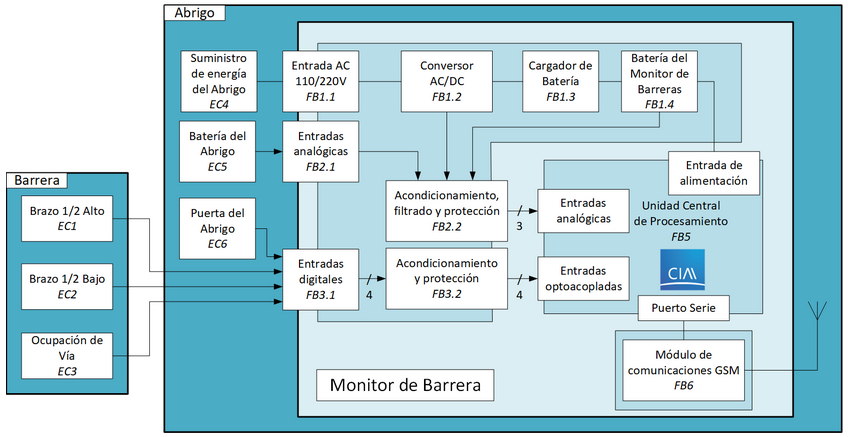
\includegraphics[width=.5\textwidth]{./Figuras/diagBloques.png}
% \caption{Diagrama en bloques del sistema}
% \label{fig:diagBloques}
% \end{figure}

% \vspace{25px}

% El tamaño de la tipografía en TODAS las figuras debe ser adecuado para que NO pase lo que ocurre acá, donde el lector debe esforzarse para poder leer el texto. Los colores usados en el diagrama deben ser adecuados, tal que ayuden a comprender mejor el diagrama, preferentemente en la gama de colores pastel.
% \end{consigna}

La navegación autónoma ha sido un tema de investigación activo durante décadas, pero recientemente ha ganado una atención sin precedentes gracias a los avances en tecnologías como la inteligencia artificial y la robótica.

La navegación autónoma se refiere a la capacidad de un sistema para planificar y ejecutar sus propias acciones de manera autónoma, sin la necesidad de una intervención humana constante.

La capacidad de un sistema para tomar decisiones en forma autónoma en su navegación a través del entorno es crucial para una amplia gama de aplicaciones, desde los vehículos autónomos y los drones, hasta los robots industriales y los sistemas de logística.

La investigación de técnicas de bajo costo es importante para permitir que la tecnología sea accesible para un mayor número de aplicaciones y usuarios. Esto es especialmente importante en países en desarrollo o en áreas con recursos limitados, donde los sistemas de navegación autónoma pueden ser prohibitivamente costosos. 

La restricción económica en el desarrollo de nuevas técnicas también puede mejorar la eficiencia y la efectividad de los sistemas de navegación autónoma, al permitir que los recursos sean utilizados de manera más efectiva y maximizar la vida útil de los componentes del sistema.

La odometría visual es una técnica de localización y navegación que se utiliza en robótica para estimar la posición y orientación de un robot en su entorno en función de la información visual capturada por sus cámaras. La información de las imágenes capturadas permite estimar la cantidad de movimiento y la dirección del vehículo, posibilitando calcular su posición y orientación en relación con su posición inicial.

Las técnicas de odometría visual son particularmente útiles en entornos donde el movimiento del robot es predominantemente lateral. Además, se pueden utilizar en combinación con otras técnicas de localización y navegación, como la odometría inercial o la SLAM (\textit{Simultaneous Localization and Mapping}), para mejorar la precisión y la fiabilidad de la localización del robot.

La SLAM es una técnica de visión por computadora que permite a un robot móvil construir un mapa del entorno en el que se encuentra, mientras simultáneamente estima su propia posición y orientación en ese entorno. En el caso de SLAM monocular, se utiliza una única cámara para capturar imágenes del entorno.

La Fundación Fulgor realiza diversas actividades de investigación. Dentro del campo de navegación autónoma, una de las ramas de interés es la de algoritmos de SLAM monocular en conjunto con la odometría inercial, por las diferentes ventajas que presenta sobre otros métodos. Se han realizado experimentos, implementando y comparando el desempeño de diferentes algoritmos en entornos de simulación.

Actualmente, uno de los objetivos en esta línea de investigación es poder migrar los algoritmos estudiados en un entorno virtual a un sistema físico, para evaluar su desempeño en un entorno real. La experimentación en entornos virtuales se llevó a cabo con el framework ROS 2 (Robot Operating System 2).
Dada la naturaleza modular de este framework, la migración consiste en el reemplazo de un módulo encapsulado que contenga el algoritmo, como se observa en la Figura \ref{fig:ros2-to-microros}. 

\begin{figure}[htpb]
\centering 
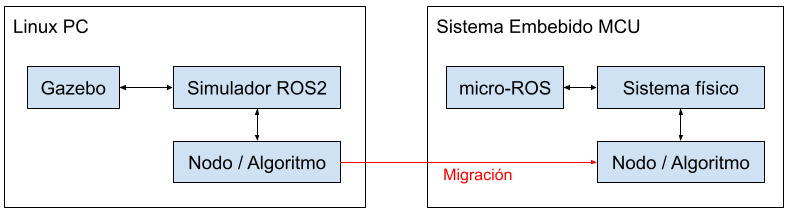
\includegraphics[width=.8\textwidth]{./Figuras/ros2-microros-migration.png}
\caption{Migración de algoritmos en entorno de simulación a sistema físico}
\label{fig:ros2-to-microros}
\end{figure}

% El uso de micro-ROS permite continuar con el uso de todas las herramientas que facilita ROS 2, manteniendo el entorno de estudio del sistema, e inclusive posibilitando la realimentación del sistema físico hacia el entorno de simulación.

El entorno ROS es un framework de software libre y de código abierto diseñado para permitir el desarrollo de aplicaciones robóticas distribuidas. Proporciona un conjunto de herramientas para la creación, gestión, depuración y análisis de sistemas robóticos.

La segunda versión de la herramienta, denominada ROS 2, fue desarrollada por la comunidad con el objetivo de mejorar la escalabilidad, la fiabilidad y la seguridad del software.
Una de sus principales características es que está diseñado para ser modular y extensible, lo que significa que los desarrolladores pueden elegir los componentes que necesitan para sus aplicaciones y utilizarlos de manera flexible. 
También se enfoca en proporcionar una abstracción de hardware más clara y permitir el uso de diferentes sistemas operativos y arquitecturas. 

La herramienta micro-ROS es una implementación de ROS 2 diseñada específicamente para sistemas embebidos y de tiempo real. A diferencia de ROS 2, que se ejecuta en sistemas operativos de propósito general, micro-ROS se ejecuta en sistemas operativos de tiempo real, como NuttX y FreeRTOS, lo que permite el desarrollo de sistemas robóticos en entornos de baja potencia y recursos limitados.

Como puede observarse en la Figura \ref{fig:microROSarch}, micro-ROS proporciona una capa de abstracción que permite la comunicación entre los sistemas embebidos y los nodos de ROS 2 en otros sistemas.
Esto significa que los desarrolladores pueden crear sistemas robóticos distribuidos, que utilicen tanto sistemas embebidos como sistemas de propósito general y que todos ellos pueden comunicarse a través de la misma plataforma.

\begin{figure}[htpb]
\centering 
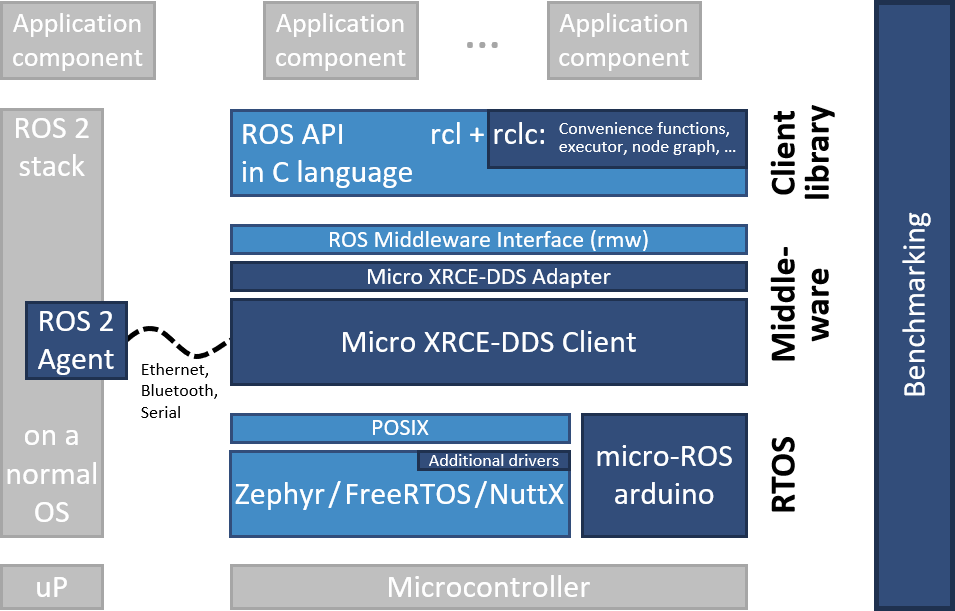
\includegraphics[width=.7\textwidth]{./Figuras/micro-ROS_architecture.png}
\caption{Arquitectura de micro-ROS}
\label{fig:microROSarch}
\end{figure}

\section{2. Identificación y análisis de los interesados}
\label{sec:interesados}

% \begin{consigna}{red} % este comando se debe borrar para la entrega, junto con la contraparte \end{consigna}{red} 
 
% \textbf{Nota importante:} borrar esto y todas las consignas en color rojo antes de entregar este documento). Esto se hace eliminando el par de comandos que forman el bloque consigna, \verb!\begin{consigna}{red}! y \verb!\end{consigna}{red}! del código. 
 
% Es inusual que una misma persona esté en más de un rol, incluso en proyectos chicos. Si se considera que una persona cumple dos o más roles, entonces solo dejarla en el rol más importante. 

% Por ejemplo, si una persona es Cliente pero también colabora u orienta, dejarla solo como Cliente. Si una persona es el Responsable, no debe ser colocado también como miembro del equipo.


% \begin{table}[ht]
% %\caption{Identificación de los interesados}
% %\label{tab:interesados}
% \begin{tabularx}{\linewidth}{@{}|l|X|X|l|@{}}
% \hline
% \rowcolor[HTML]{C0C0C0} 
% Rol           & Nombre y Apellido & Organización 	& Puesto 	\\ \hline
% Auspiciante   &                   &              	&        	\\ \hline
% Cliente       & \clientename      &\empclientename	&        	\\ \hline
% Impulsor      &                   &              	&        	\\ \hline
% Responsable   & \authorname       & FIUBA        	& Alumno 	\\ \hline
% Colaboradores &                   &              	&        	\\ \hline
% Orientador    & \supname	      & \pertesupname 	& Director Trabajo final \\ \hline
% Equipo        & miembro1 \newline 
% 				miembro2          &              	&        	\\ \hline
% Opositores    &                   &              	&        	\\ \hline
% Usuario final &                   &              	&        	\\ \hline
% \end{tabularx}
% \end{table}

% El Director suele ser uno de los Orientadores.

% No dejar celdas vacías; si no hay nada que poner en una celda colocar un signo ``-''.

% No dejar filas vacías; si no hay nada que poner en una fila entonces eliminarla.

% Es deseable listar a continuación las principales características de cada interesado.
 
% Por ejemplo:
% \begin{itemize}
% 	\item Auspiciante: es riguroso y exigente con la rendición de gastos. Tener mucho cuidado con esto.
% 	\item Equipo: Juan Perez, suele pedir licencia porque tiene un familiar con una enfermedad. Planificar considerando esto.
% 	\item Orientador: María Gómez va a poder ayudar mucho con la definición de los requerimientos.
% \end{itemize}

% \end{consigna} % este comando se debe borrar para la entrega, junto con la contraparte \begin{consigna}{red}

\begin{itemize}
	\item Cliente: El \clientename{} tiene se encuentra haciendo su doctorado en la Fundación Fulgor y posee un gran conocimiento sobre los algoritmos utilizados para navegación autónoma a alto nivel. Es capaz de resolver dudas específicas sobre los requerimientos a cumplir con el algoritmo a implementar.
	\item Equipo: Evangelina Castellano se encuentra realizando su Práctica Profesional Supervisada (PPS) en la Fundación Fulgor. Al finalizar su PPS continuará en la institución para realizar su proyecto final de grado. Es necesario planificar teniendo en cuenta que la dedicación es simple, es decir, entre 4 y 5 horas diarias.
	\item Usuario final: No esta representado por una persona particular. Una vez finalizado el proyecto el prototipo quedará disponible en la Fundación Fulgor para su uso.
\end{itemize}

\begin{table}[ht]
%\caption{Identificación de los interesados}
%\label{tab:interesados}
\begin{tabularx}{\linewidth}{@{}|l|X|X|l|@{}}
\hline
\rowcolor[HTML]{C0C0C0} 
Rol           & Nombre y Apellido & Organización 	& Puesto 	\\ \hline
% Auspiciante   &                   &              	&        	\\ \hline
Cliente       & \clientename      &\empclientename	&  Investigador      	\\ \hline
% Impulsor      &                   &              	&        	\\ \hline
Responsable   & \authorname       & FIUBA        	& Alumno 	\\ \hline
% Colaboradores &                   &              	&        	\\ \hline
Orientador    & \supname	      & \pertesupname 	& Director Trabajo final \\ \hline
Equipo        & Evangelina Castellano          &        Universidad Nacional de Córdoba    	&     Colaboradores   	\\ \hline
%Opositores    &                   &              	&        	\\ \hline
Usuario final & Grupos de investigación                  &   Fundación Fulgor           	&     -   	\\ \hline
\end{tabularx}
\end{table}

\section{3. Propósito del proyecto}
\label{sec:proposito}

El propósito de este proyecto es desarrollar el prototipo de una plataforma de hardware con las capacidades para poder implementar los algoritmos investigados de SLAM monocular y observar resultados.

La técnica de SLAM monocular es de interés por su aplicación en la navegación autónoma de vehículos, su bajo costo económico y simpleza del hardware involucrado en comparación a otras técnicas utilizadas en el área.

\section{4. Alcance del proyecto}
\label{sec:alcance}

% \begin{consigna}{red}
% ¿Qué se incluye y que no se incluye en este proyecto?

% Se refiere al trabajo a hacer para entregar el producto o resultado especificado. 

% Explicitar todo lo quede comprendido dentro del alcance del proyecto.

% Explicitar además todo lo que no quede incluido (``El presente proyecto no incluye...'')

% \end{consigna}

El proyecto incluye el diseño del sistema embebido, el desarrollo de los drivers de los sensores asociados a las técnicas de SLAM monocular, la incorporación de la interfaz de micro-ROS en el proyecto, la aplicación de ROS 2 que permitirá interactuar con el sistema a alto nivel y la investigación e implementación de un algoritmo de SLAM monocular adecuado.

El proyecto no incluye el desarrollo de algoritmos de navegación autónoma asociados a la planificación y ejecución de trayectorias del vehículo ni el modelado matemático del mismo. Tampoco incluye optimización de los algoritmos planteados con el uso de hardware dedicado como una FPGA, por ser una actividad que se realizará en una segunda etapa del proyecto.

Por lo tanto, el producto final esperado es un prototipo de un sistema embebido con los correspondientes sensores y herramientas necesarias funcionando en conjunto con técnicas de SLAM monocular, que un vehículo móvil pueda incorporar para dotarlo con capacidades de navegación autónoma.

\section{5. Supuestos del proyecto}
\label{sec:supuestos}

% \begin{consigna}{red}
% ``Para el desarrollo del presente proyecto se supone que: ...''

% \begin{itemize}
% 	\item Supuesto 1
% 	\item Supuesto 2...
% \end{itemize}

% Por ejemplo, se podrían incluir supuestos respecto a disponibilidad de tiempo y recursos humanos y materiales, sobre la factibilidad técnica de distintos aspectos del proyecto, sobre otras cuestiones que sean necesarias para el éxito del proyecto como condiciones macroeconómicas o reglamentarias.
% \end{consigna}

Para el desarrollo del presente proyecto se supone que:

\begin{itemize}
	\item La adquisición de materiales no tendrá demoras mayores a una semana, asumiendo que el mercado local posee los materiales requeridos para la fabricación del prototipo.
	\item No habrán cambios en el equipo de trabajo en el periodo de tiempo que comprende la planificación del proyecto.
	\item El responsable del proyecto puede dedicar una cantidad mínima de 25 horas semanales a las actividades del plan.
	\item El responsable del proyecto estará ausente durante dos semanas de Julio del año 2023, con fecha a definir.
	\item No habrán cambios en los objetivos principales del proyecto ni nuevos requerimientos funcionales de parte del cliente.
\end{itemize}

\section{6. Requerimientos}
\label{sec:requerimientos}

% \begin{consigna}{red}
% Los requerimientos deben numerarse y de ser posible estar agruparlos por afinidad, por ejemplo:

% \begin{enumerate}
% 	\item Requerimientos funcionales
% 		\begin{enumerate}
% 			\item El sistema debe...
% 			\item Tal componente debe...
% 			\item El usuario debe poder...
% 		\end{enumerate}
% 	\item Requerimientos de documentación
% 		\begin{enumerate}
% 			\item Requerimiento 1
% 			\item Requerimiento 2 (prioridad menor)
% 		\end{enumerate}
% 	\item Requerimiento de testing...
% 	\item Requerimientos de la interfaz...
% 	\item Requerimientos interoperabilidad...
% 	\item etc...
% \end{enumerate}

% Leyendo los requerimientos se debe poder interpretar cómo será el proyecto y su funcionalidad.

% Indicar claramente cuál es la prioridad entre los distintos requerimientos y si hay requerimientos opcionales. 

% No olvidarse de que los requerimientos incluyen a las regulaciones y normas vigentes!!!

% Y al escribirlos seguir las siguientes reglas:
% \begin{itemize}
% 	\item Ser breve y conciso (nadie lee cosas largas). 
% 	\item Ser específico: no dejar lugar a confusiones.
% 	\item Expresar los requerimientos en términos que sean cuantificables y medibles.
% \end{itemize}

% \end{consigna}

\subsection{Requerimientos funcionales}
\begin{itemize}
	\item El driver de la Unidad de Medición Inercial (IMU por sus siglas en inglés) debe ofrecer a la aplicación la información del giróscopo y acelerómetro de forma completa. Se deben brindar todas las posibilidades de configuración necesarias para poder adaptar la escala y frecuencia de muestreo de los sensores a los requisitos de la aplicación. El driver debe implementarse de forma modular para que pueda utilizarse independientemente del proyecto.
	\item El driver de la cámara debe proveer a la aplicación la información correcta dadas las capacidades del dispositivo.
	\item El sistema embebido debe utilizar micro-ROS para interactuar e integrarse fácilmente con el entorno de desarrollo, monitoreo y evaluación de ROS 2.
	\item El sistema embebido debe hacer un uso adecuado de los mecanismos de comunicación de micro-ROS con ROS 2 para explotar todas las ventajas que ofrece el framework.
	\item El sistema debe estar diseñado de forma modular para favorecer su escalabilidad.
	\item El sistema debe utilizar algoritmos y técnicas de fusión sensorial para optimizar el uso de la información obtenida por la IMU.
	\item El sistema debe ejecutar un algoritmo investigado previamente de SLAM monocular.
\end{itemize}

\subsection{Requerimientos de documentación}
\begin{itemize}
	\item Todas aquellas funcionalidades cubiertas en el driver de la IMU deben estar completamente documentadas para que el módulo de software pueda utilizarse independientemente del proyecto.
	\item El proceso de incorporación y uso de las librerías de micro-ROS debe estar correctamente documentado para facilitar el desarrollo continuo del sistema.
	\item La investigación del estado del arte en el tópico de algoritmos de SLAM monocular debe estar debidamente documentada.
	\item El algoritmo seleccionado para implementar en el sistema debe estar documentado en forma detallada.
\end{itemize}

\subsection{Requerimientos de testing}
\begin{itemize}
	\item Se deben aplicar herramientas y metodologías de testing en los drivers de los módulos para asegurar su funcionamiento y calidad.
\end{itemize}

\subsection{Requerimientos de la interfaz}
\begin{itemize}
	\item Las herramientas desarrolladas en el entorno de ROS 2 deben también cumplir el propósito de interfaz gráfica y permitir la visualización de la información obtenida a través de los sensores.
	\item El sistema desarrollado con ROS 2 debe ofrecer herramientas que permitan operar y reconfigurar el sistema.
	\item El sistema desarrollado con ROS 2 debe ofrecer herramientas que permitan evaluar de forma sencilla el desempeño del algoritmo implementado.
\end{itemize}

\section{7. Historias de usuarios (\textit{Product backlog})}
\label{sec:backlog}

Se identifican los siguientes roles/usuarios:
\begin{enumerate}
	\item Investigador en el área de Ciencias de la Computación, en su rol de estudiante de máster o PhD desea realizar avances en los algoritmos de navegación autónoma. No necesariamente tiene conocimientos de electrónica y sistemas embebidos, su foco es el desarrollo a alto nivel.
	\item Investigador en el área de la electrónica, sistemas embebidos y/o firmware, en su rol de estudiante de máster o PhD desea realizar avances en el desarrollo de dispositivos de navegación autónoma mediante la optimización o mejora del hardware y el firmware asociado.
	\item Usuario perteneciente a la comunidad de código abierto/libre, en su rol desea implementar el proyecto con sus propios materiales, aplicarlo en un caso de uso específico y colaborar con posibles mejoras. Puede o no poseer conocimiento técnico.
\end{enumerate}

La ponderación de cada historia de usuario se obtiene de una evaluación sobre tres ejes: tiempo, dificultad e incertidumbre. Sobre cada eje se asigna un valor en una escala entre 0 y 5, luego este valor se penaliza según la relevancia asignada a cada aspecto: tiempo 0.4, dificultad 0.2 e incertidumbre 0.4. Para obtener el puntaje final de la historia se divide el resultado parcial por 5 y se multiplica por 100.

\textbf{Historia 1 de usuario 1:} como investigador en el área de Ciencias de la Computación quiero poder utilizar los sensores de SLAM monocular como si fueran una caja negra, quiero que sea sencillo aprender a utilizarlo e incorporarlo en mi flujo de trabajo para bajar de forma sencilla al dispositivo los algoritmos implementados a alto nivel en la simulación.

Tiempo: 4. Dificultad: 3. Incertidumbre: 2. Puntaje: 60 

\textbf{Historia 2 de usuario 1:} como investigador en el área de Ciencias de la Computación quiero poder visualizar la información obtenida por los sensores y utilizarla como entrada a simulaciones virtuales.

Tiempo: 3. Dificultad: 2. Incertidumbre: 1. Puntaje: 40 

\textbf{Historia 1 de usuario 2:} como investigador en el área de la electrónica quiero poder entender rápido cómo esta conformado el sistema y que sea lo suficientemente modular como para modificar, mejorar y/o intercambiar algún componente funcional y que el sistema siga operando sin dificultades.
% Un ejemplo puede ser la incorporación de una FPGA como hardware dedicado para optimizar alguna etapa del algoritmo.

Tiempo: 4. Dificultad: 3. Incertidumbre: 2. Puntaje: 60

\textbf{Historia 2 de usuario 2:} como investigador en el área de la electrónica quiero poder reutilizar los componentes que conforman el sistema de forma independiente en un proyecto diferente.

Tiempo: 3. Dificultad: 3. Incertidumbre: 2. Puntaje: 52

\textbf{Historia 1 de usuario 3:} como parte de la comunidad de código abierto/libre quiero que los materiales utilizados en el prototipo sean accesibles y que el proyecto tenga la documentación completa de las distintas etapas para poner en marcha el sistema.

Tiempo: 5. Dificultad: 1. Incertidumbre: 3. Puntaje: 68

\textbf{Historia 2 de usuario 3:} como parte de la comunidad de código abierto/libre quiero que el proyecto posea un mecanismo para poder contribuir en cualquiera de sus aspectos dado mi conocimiento específico.

Tiempo: 4. Dificultad: 2. Incertidumbre: 3. Puntaje: 64

\section{8. Entregables principales del proyecto}
\label{sec:entregables}

Los entregables del proyecto son:
\begin{itemize}
	\item Plataforma de hardware que conforma el prototipo funcional
	\item Documentación del hardware e interconexión de los módulos componentes
	\item Código fuente del driver de la IMU
	\item Documentación del driver de la IMU
	\item Código fuente del driver de la cámara
	\item Documentación del driver de la cámara
	\item Código fuente del firmware con el algoritmo de SLAM monocular y micro-ROS
	\item Código fuente del agente de ROS 2 utilizado
	\item Documentación y manual para configuración y uso del entorno de ROS 2
	\item Documentación del estado del arte de SLAM y del algoritmo seleccionado
	\item Manual de uso del hardware
	\item Informe final
\end{itemize}

\section{9. Desglose del trabajo en tareas}
\label{sec:wbs}

\begin{itemize}
	\item Setup del entorno de trabajo para desarrollo del software necesario (5h)
	\item Implementación de micro-ROS en el sistema embebido (total: 18h)
	\begin{enumerate}
		\item Introducción a micro-ROS (4h)
		\item Incorporación de micro-ROS en el microcontrolador (8h)
		\item Setup de agente de ROS 2 y comunicación con sistema embebido (2h)
		\item Documentación del proceso (4h)
	\end{enumerate}
	\item Desarrollo de driver para la IMU (total: 40h)
	\begin{enumerate}
		\item Selección y adquisición de la IMU a utilizar (2h)
		\item Implementación de driver en lenguaje C para el sistema embebido (30h)
		\item Documentación del driver (8h)
	\end{enumerate}
	\item Integración de la IMU en el sistema (total: 60h)
	\begin{enumerate}
		\item Integración de driver de la IMU con el sistema con micro-ROS (4h)
		\item Repaso (e investigación) de técnicas de fusión sensorial (8h)
		\item Implementación de algoritmos de fusión sensorial (30h)
		\item Visualización de la información obtenida con la IMU mediante las herramientas de ROS 2 (10h)
		\item Evaluación parcial de resultados y documentación de los mismos (milestone) (8h)
	\end{enumerate}
	\item Desarrollo de driver para la cámara (total: 53h)
	\begin{enumerate}
		\item Selección y adquisición de cámara a utilizar (3h)
		\item Implementación de driver en lenguaje C para el sistema embebido (40h)
		\item Documentación del driver (10h)
	\end{enumerate}
	\item Integración de la cámara en el sistema (26h)
	\begin{enumerate}
		\item Integración del driver de la cámara con el sistema con micro-ROS (6h)
		\item Visualización de la información obtenida con la cámara mediante las herramientas de ROS 2 (12h)
		\item Evaluación parcial de resultados y documentación de los mismos (milestone) (8h)
	\end{enumerate}
	\item Implementación de algoritmo de SLAM monocular (345h)
	\begin{enumerate}
		\item Introducción a navegación inercial y SLAM monocular, investigación de estado del arte (15h)
		\item Investigación de algoritmos de SLAM monocular y selección de uno a implementar (30h)
		\item Implementación del algoritmo seleccionado en un entorno de simulación (80h)
		\item Evaluación integral de los componentes del sistema (20h)
		\item Implementación del algoritmo seleccionado sobre la plataforma desarrollada (120h)
		\item Evaluación final de resultados (milestone) (40h)
		\item Documentación técnica del algoritmo seleccionado y resumen del estado del arte (40h)
	\end{enumerate}
	\item Elaboración de memoria técnica (80h)
\end{itemize}

Cantidad total de horas: 627h

% Please add the following required packages to your document preamble:
% \usepackage{booktabs}
\begin{table}[]
\caption{WBS: Desglose del trabajo en tareas}
\label{tab:wbs}
\begin{tabular}{@{}llll@{}}
\toprule
\textbf{Código} & \textbf{Predecesora} & \textbf{Descripción}                               & \textbf{Duración} \\ \midrule
1               &                      & Setup del entorno de trabajo                       & 5h                \\
2               &                      & Implementación de micro-ROS                        & 18h               \\
2.1             &                      & Introducción a micro-ROS                           & 4h                \\
2.2             & 1, 2.1               & Incorporación de micro-ROS en el sistema           & 8h                \\
2.3             & 2.2                  & Setup del agente de ROS 2                          & 2h                \\
2.4             & 2.3                  & Documentación del proceso                          & 4h                \\
3               &                      & Desarrollo de driver para la IMU                   & 40h               \\
3.1             &                      & Selección y adquisición de la IMU a utilizar       & 2h                \\
3.2             & 1, 3.1               & Implementación de driver para el sistema embebido  & 30h               \\
3.3             & 3.2                  & Documentación del driver                           & 8h                \\
4               &                      & Integración de la IMU en el sistema                & 60h               \\
4.1             & 2.3, 3.2             & Integración del driver de la IMU con micro-ROS     & 4h                \\
4.2             &                      & Repaso de técnicas de fusión sensorial             & 8h                \\
4.3             & 3.2, 4.2             & Implementación de algoritmos de fusión sensorial   & 30h               \\
4.4             & 4.1                  & Visualización de la información mediante ROS 2     & 10h               \\
4.5             & 4.3, 4.4             & Evaluación parcial de resultados y documentación   & 8h                \\
5               &                      & Desarrollo de driver para la cámara                & 53h               \\
5.1             &                      & Selección y adquisición de la cámara a utilizar    & 3h                \\
5.2             & 1, 5.1               & Implementación de driver para el sistema embebido  & 40h               \\
5.3             & 5.2                  & Documentación del driver                           & 10h               \\
6               &                      & Integración de la cámara en el sistema             & 26h               \\
6.1             & 2.3, 5.2             & Integración del driver de la cámara con micro-ROS  & 6h                \\
6.2             & 6.1                  & Visualización de la información mediante ROS 2     & 12h               \\
6.3             & 6.2                  & Evaluación parcial de resultados y documentación   & 8h                \\
7               &                      & Implementación de algoritmo de SLAM monocular      & 345h              \\
7.1             &                      & Investigación del estado del arte de SLAM          & 15h               \\
7.2             & 7.1                  & Investigación y selección de algoritmos de SLAM    & 30h               \\
7.3             & 1, 7.2               & Implementación del algoritmo en simulación         & 80h               \\
7.4             & 4.5, 6.3        & Evaluación integral de los componentes del sistema & 20h               \\
7.5             & 7.3, 7.4                  & Implentación del algoritmo en el sistema embebido  & 120h              \\
7.6             & 7.5                  & Evaluación final de resultados                     & 40h               \\
7.7             & 7.6                  & Documentación técnica del algoritmo                & 50h               \\
8               & 7.6                  & Elaboración de memoria técnica                     & 80h               \\ \bottomrule
\end{tabular}
\end{table}

\section{10. Diagrama de Activity On Node}
\label{sec:AoN}

% \begin{consigna}{red}
% Armar el AoN a partir del WBS definido en la etapa anterior. 

%La figura \ref{fig:AoN} fue elaborada con el paquete latex tikz y pueden consultar la siguiente referencia \textit{online}:

%\url{https://www.overleaf.com/learn/latex/LaTeX_Graphics_using_TikZ:_A_Tutorial_for_Beginners_(Part_3)\%E2\%80\%94Creating_Flowcharts}

% \end{consigna}


\begin{landscape}
\begin{figure}[htpb]
\centering 
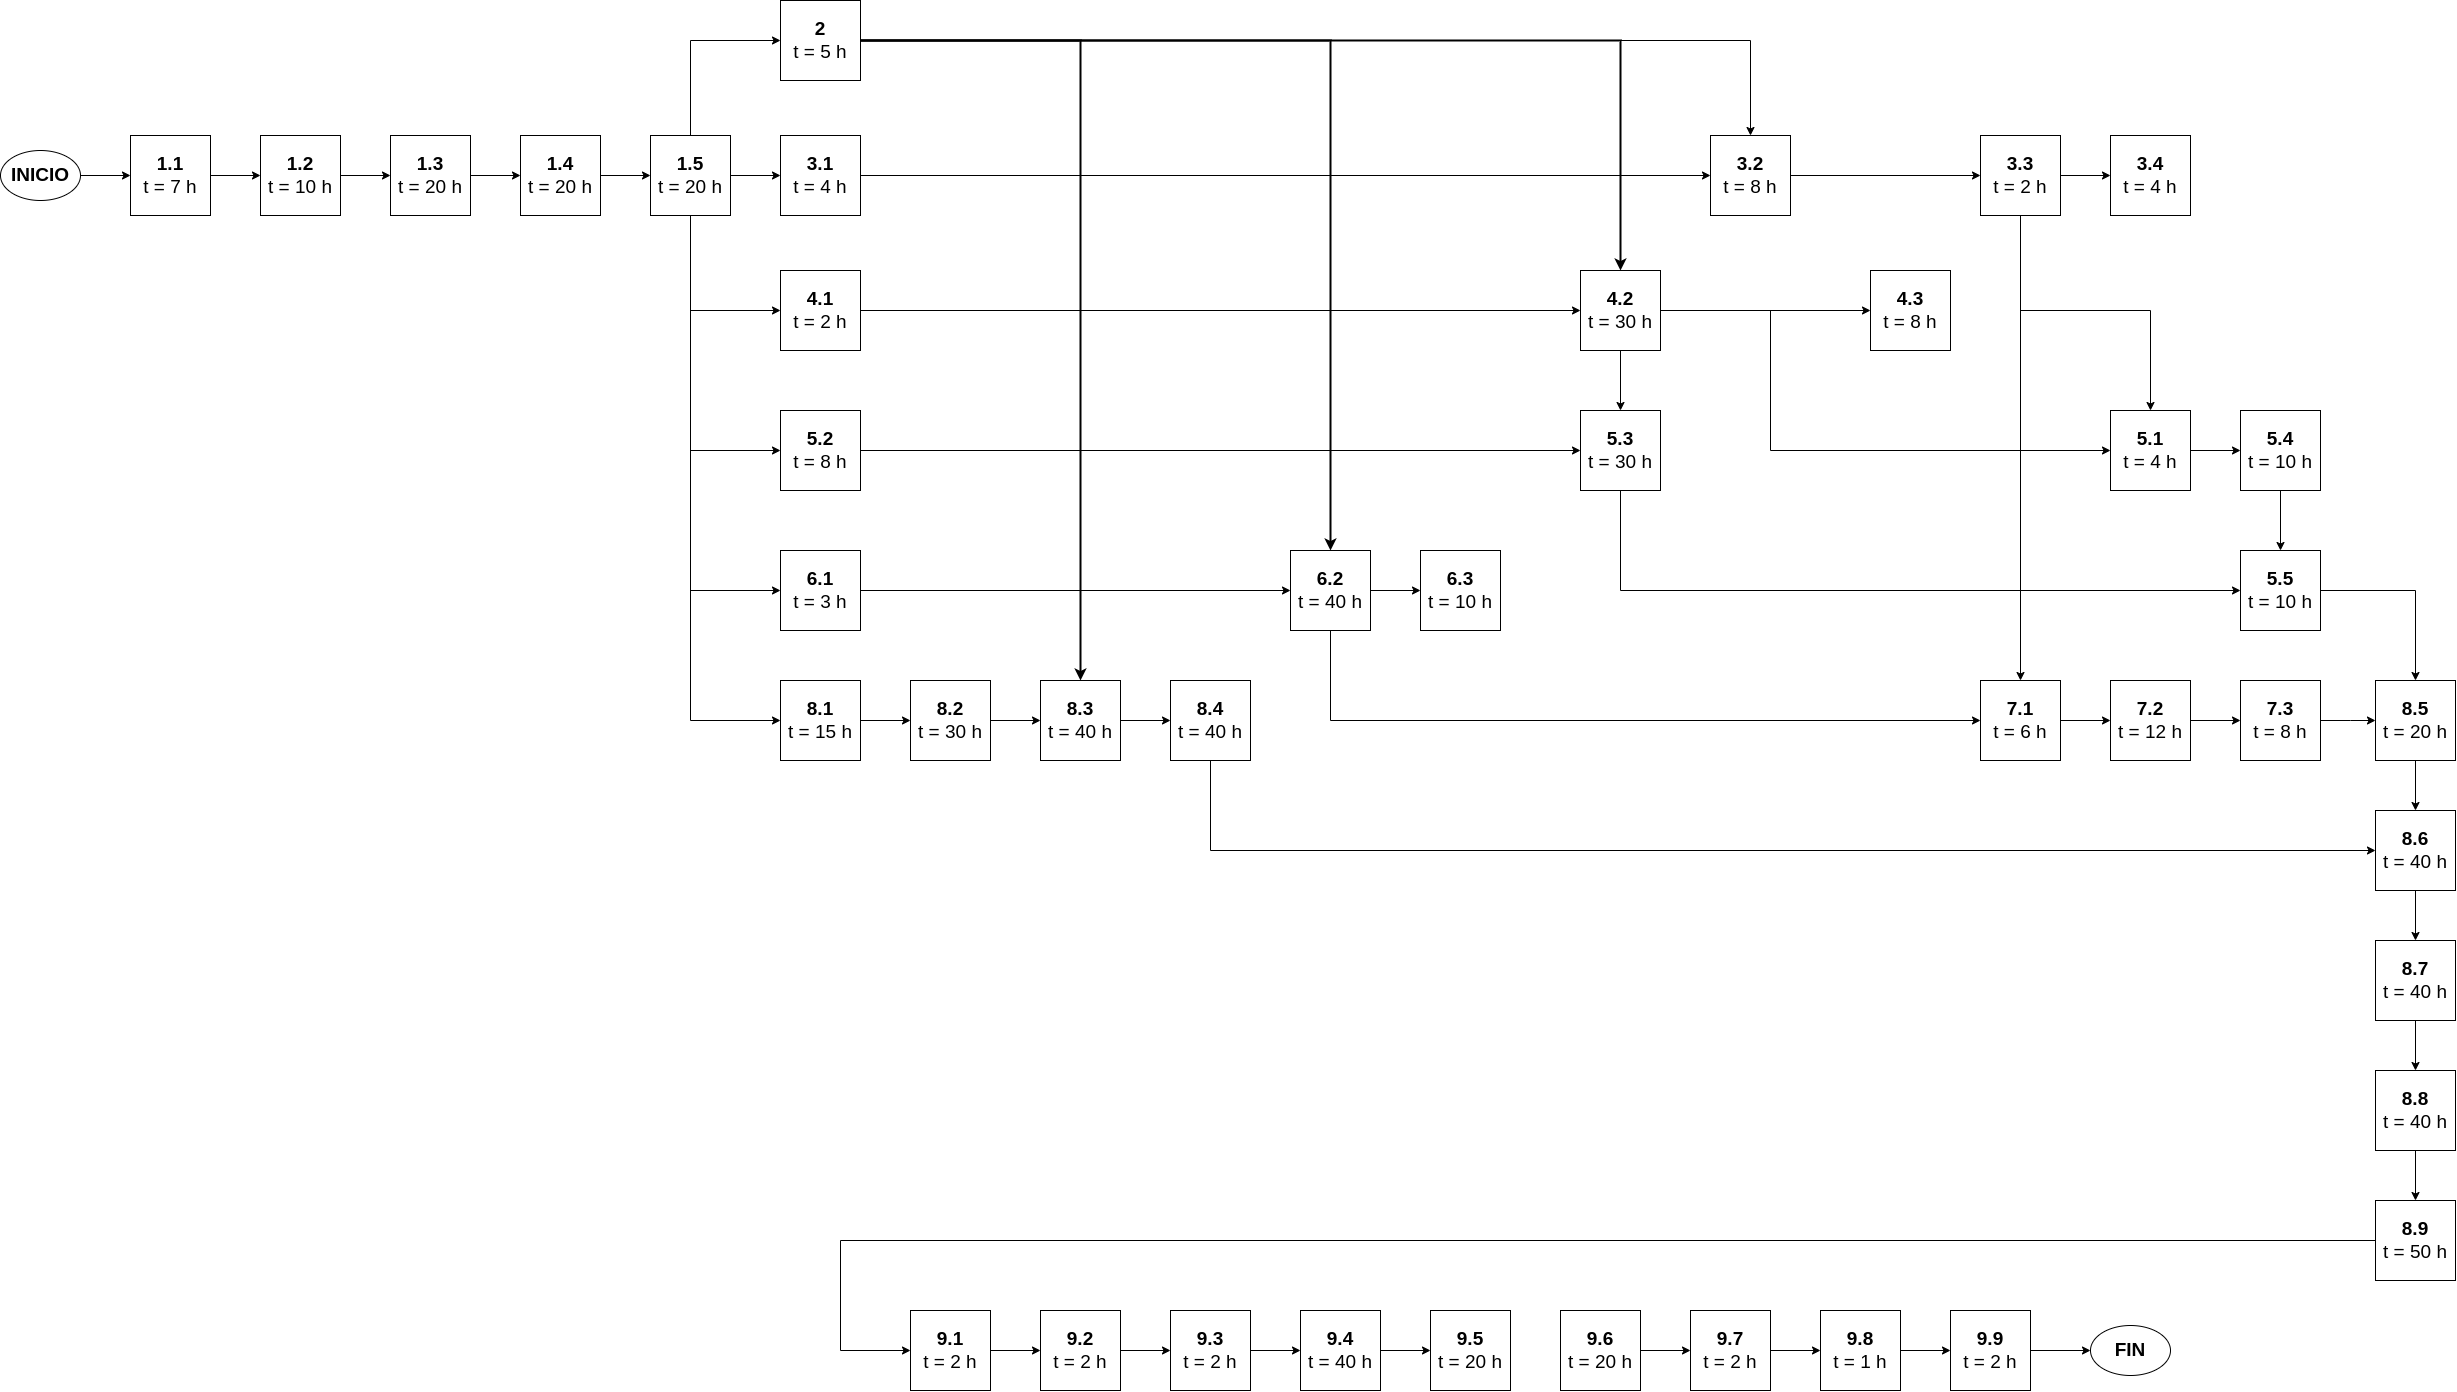
\includegraphics[width=1.5\textwidth]{./Figuras/MonoSLAM-AoN.png}
\caption{Diagrama de \textit{Activity on Node}.}
\label{fig:AoN}
\end{figure}
\end{landscape}

% Indicar claramente en qué unidades están expresados los tiempos.
% De ser necesario indicar los caminos semicríticos y analizar sus tiempos mediante un cuadro.
% Es recomendable usar colores y un cuadro indicativo describiendo qué representa cada color, como se muestra en el siguiente ejemplo:



\section{11. Diagrama de Gantt}
\label{sec:gantt}

% \begin{consigna}{red}

% Existen muchos programas y recursos \textit{online} para hacer diagramas de Gantt, entre los cuales destacamos:

% \begin{itemize}
% \item Planner
% \item GanttProject
% \item Trello + \textit{plugins}. En el siguiente link hay un tutorial oficial: \\ \url{https://blog.trello.com/es/diagrama-de-gantt-de-un-proyecto}
% \item Creately, herramienta online colaborativa. \\\url{https://creately.com/diagram/example/ieb3p3ml/LaTeX}
% \item Se puede hacer en latex con el paquete \textit{pgfgantt}\\ \url{http://ctan.dcc.uchile.cl/graphics/pgf/contrib/pgfgantt/pgfgantt.pdf}
% \end{itemize}

% Pegar acá una captura de pantalla del diagrama de Gantt, cuidando que la letra sea suficientemente grande como para ser legible. 
% Si el diagrama queda demasiado ancho, se puede pegar primero la ``tabla'' del Gantt y luego pegar la parte del diagrama de barras del diagrama de Gantt.

% Configurar el software para que en la parte de la tabla muestre los códigos del EDT (WBS).\\
% Configurar el software para que al lado de cada barra muestre el nombre de cada tarea.\\
% Revisar que la fecha de finalización coincida con lo indicado en el Acta Constitutiva.

% En la figura \ref{fig:gantt}, se muestra un ejemplo de diagrama de Gantt realizado con el paquete de \textit{pgfgantt}. En la plantilla pueden ver el código que lo genera y usarlo de base para construir el propio.

% \begin{figure}[htbp]
% \begin{center}
% \begin{ganttchart}{1}{12}
%   \gantttitle{2020}{12} \\
%   \gantttitlelist{1,...,12}{1} \\
%   \ganttgroup{Group 1}{1}{7} \\
%   \ganttbar{Task 1}{1}{2} \\
%   \ganttlinkedbar{Task 2}{3}{7} \ganttnewline
%   \ganttmilestone{Milestone o hito}{7} \ganttnewline
%   \ganttbar{Final Task}{8}{12}
%   \ganttlink{elem2}{elem3}
%   \ganttlink{elem3}{elem4}
% \end{ganttchart}
% \end{center}
% \caption{Diagrama de Gantt de ejemplo}
% \label{fig:gantt}
% \end{figure}


% \begin{landscape}
% \begin{figure}[htpb]
% \centering 
% 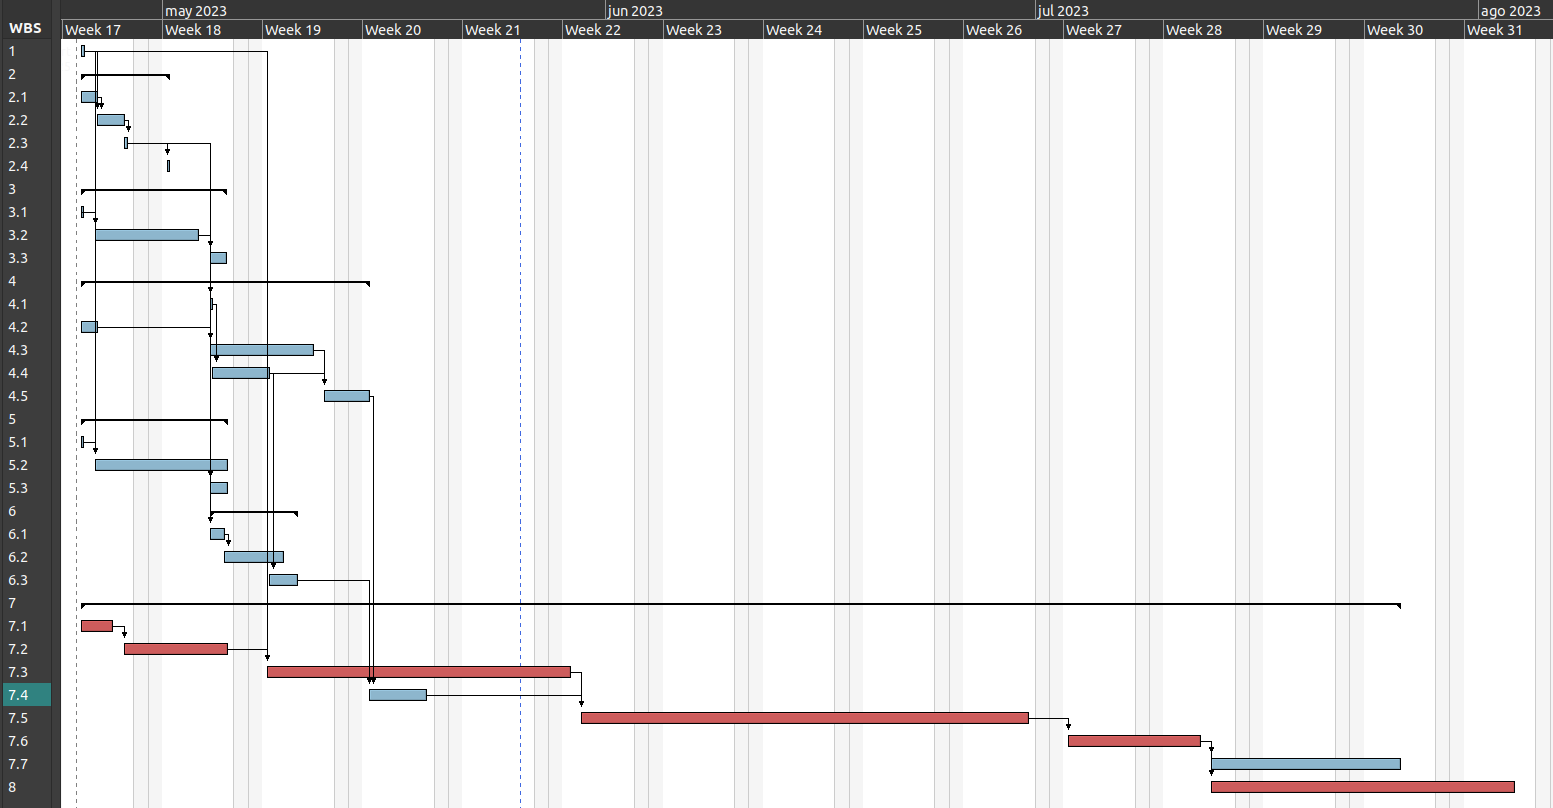
\includegraphics[height=.85\textheight]{./Figuras/Gantt_v1.png}
% \caption{Ejemplo de diagrama de Gantt rotado}
% \label{fig:diagGantt}
% \end{figure}
% \end{landscape}

% \end{consigna}

\begin{landscape}
\begin{figure}[htpb]
\centering 
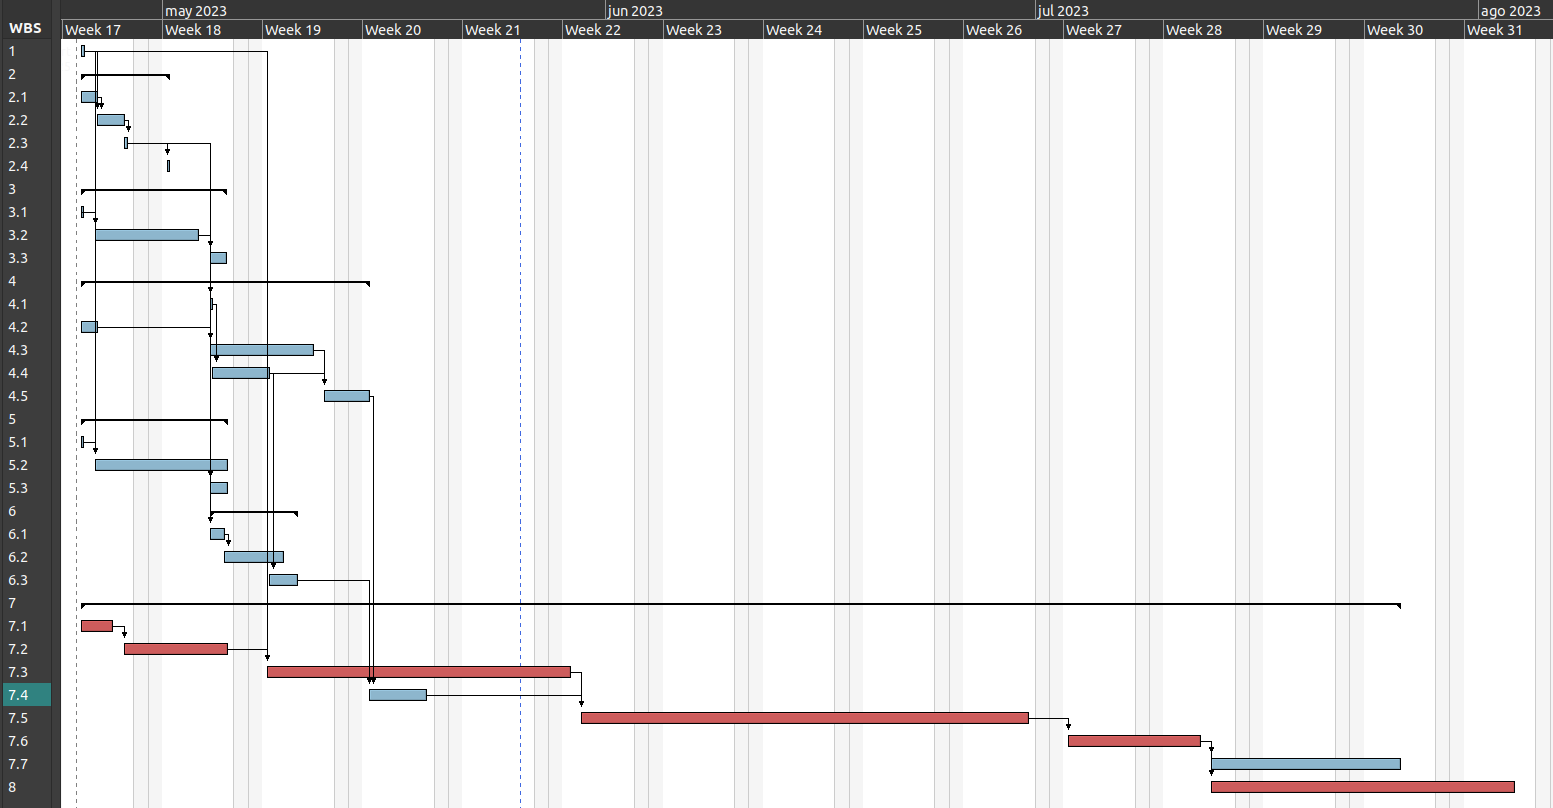
\includegraphics[height=.8\textheight]{./Figuras/Gantt_v1.png}
\caption{Diagrama de Gantt del proyecto}
\label{fig:diagGantt}
\end{figure}
\end{landscape}


\section{12. Presupuesto detallado del proyecto}
\label{sec:presupuesto}

% \begin{consigna}{red}
% Si el proyecto es complejo entonces separarlo en partes:
% \begin{itemize}
% 	\item Un total global, indicando el subtotal acumulado por cada una de las áreas.
% 	\item El desglose detallado del subtotal de cada una de las áreas.
% \end{itemize}

% IMPORTANTE: No olvidarse de considerar los COSTOS INDIRECTOS.

% \end{consigna}

\begin{table}[htpb]
\centering
\begin{tabularx}{\linewidth}{@{}|X|c|r|r|@{}}
\hline
\rowcolor[HTML]{C0C0C0} 
\multicolumn{4}{|c|}{\cellcolor[HTML]{C0C0C0}COSTOS DIRECTOS} \\ \hline
\rowcolor[HTML]{C0C0C0} 
Descripción &
  \multicolumn{1}{c|}{\cellcolor[HTML]{C0C0C0}Cantidad} &
  \multicolumn{1}{c|}{\cellcolor[HTML]{C0C0C0}Valor unitario} &
  \multicolumn{1}{c|}{\cellcolor[HTML]{C0C0C0}Valor total} \\ \hline
Placa de desarrollo STM32 Nucleo &
  \multicolumn{1}{c|}{1} &
  \multicolumn{1}{c|}{30000 ARS} &
  \multicolumn{1}{c|}{30000 ARS} \\ \hline
Cámara &
  \multicolumn{1}{c|}{1} &
  \multicolumn{1}{c|}{5000 ARS} &
  \multicolumn{1}{c|}{5000 ARS} \\ \hline
\multicolumn{1}{|l|}{Unidad de medición inercial} &
  \multicolumn{1}{c|}{1} &
  \multicolumn{1}{c|}{5000 ARS} &
  \multicolumn{1}{c|}{5000 ARS} \\ \hline
\multicolumn{1}{|l|}{Componentes de electrónica varios} &
  \multicolumn{1}{c|}{1} &
  \multicolumn{1}{c|}{3000 ARS} &
  \multicolumn{1}{c|}{3000 ARS} \\ \hline
\multicolumn{1}{|l|}{Hora de ingeniería} &
  \multicolumn{1}{c|}{600} &
  \multicolumn{1}{c|}{2500 ARS} &
  \multicolumn{1}{c|}{1500000 ARS} \\ \hline
\multicolumn{3}{|c|}{SUBTOTAL} &
  \multicolumn{1}{c|}{1543000 ARS} \\ \hline
\rowcolor[HTML]{C0C0C0} 
\multicolumn{4}{|c|}{\cellcolor[HTML]{C0C0C0}COSTOS INDIRECTOS} \\ \hline
\rowcolor[HTML]{C0C0C0} 
Descripción &
  \multicolumn{1}{c|}{\cellcolor[HTML]{C0C0C0}Cantidad} &
  \multicolumn{1}{c|}{\cellcolor[HTML]{C0C0C0}Valor unitario} &
  \multicolumn{1}{c|}{\cellcolor[HTML]{C0C0C0}Valor total} \\ \hline
\multicolumn{1}{|l|}{Transporte} &
  \multicolumn{1}{c|}{10} &
  \multicolumn{1}{c|}{100 ARS} &
  \multicolumn{1}{c|}{1000 ARS} \\ \hline
\multicolumn{1}{|l|}{Energía eléctrica} &
  \multicolumn{1}{c|}{1} &
  \multicolumn{1}{c|}{2000 ARS} &
  \multicolumn{1}{c|}{2000 ARS} \\ \hline
\multicolumn{3}{|c|}{SUBTOTAL} &
  \multicolumn{1}{c|}{3000 ARS} \\ \hline
\rowcolor[HTML]{C0C0C0}
\multicolumn{3}{|c|}{TOTAL} &
   \\ \hline
\end{tabularx}%
\end{table}


\section{13. Gestión de riesgos}
\label{sec:riesgos}

\begin{consigna}{red}
a) Identificación de los riesgos (al menos cinco) y estimación de sus consecuencias:
 
Riesgo 1: detallar el riesgo (riesgo es algo que si ocurre altera los planes previstos de forma negativa)
\begin{itemize}
	\item Severidad (S): mientras más severo, más alto es el número (usar números del 1 al 10).\\
	Justificar el motivo por el cual se asigna determinado número de severidad (S).
	\item Probabilidad de ocurrencia (O): mientras más probable, más alto es el número (usar del 1 al 10).\\
	Justificar el motivo por el cual se asigna determinado número de (O). 
\end{itemize}   

Riesgo 2:
\begin{itemize}
	\item Severidad (S): 
	\item Ocurrencia (O):
\end{itemize}

Riesgo 3:
\begin{itemize}
	\item Severidad (S): 
	\item Ocurrencia (O):
\end{itemize}


b) Tabla de gestión de riesgos:      (El RPN se calcula como RPN=SxO)

\begin{table}[htpb]
\centering
\begin{tabularx}{\linewidth}{@{}|X|c|c|c|c|c|c|@{}}
\hline
\rowcolor[HTML]{C0C0C0} 
Riesgo & S & O & RPN & S* & O* & RPN* \\ \hline
       &   &   &     &    &    &      \\ \hline
       &   &   &     &    &    &      \\ \hline
       &   &   &     &    &    &      \\ \hline
       &   &   &     &    &    &      \\ \hline
       &   &   &     &    &    &      \\ \hline
\end{tabularx}%
\end{table}

Criterio adoptado: 
Se tomarán medidas de mitigación en los riesgos cuyos números de RPN sean mayores a...

Nota: los valores marcados con (*) en la tabla corresponden luego de haber aplicado la mitigación.

c) Plan de mitigación de los riesgos que originalmente excedían el RPN máximo establecido:
 
Riesgo 1: plan de mitigación (si por el RPN fuera necesario elaborar un plan de mitigación).
  Nueva asignación de S y O, con su respectiva justificación:
  - Severidad (S): mientras más severo, más alto es el número (usar números del 1 al 10).
          Justificar el motivo por el cual se asigna determinado número de severidad (S).
  - Probabilidad de ocurrencia (O): mientras más probable, más alto es el número (usar del 1 al 10).
          Justificar el motivo por el cual se asigna determinado número de (O).

Riesgo 2: plan de mitigación (si por el RPN fuera necesario elaborar un plan de mitigación).
 
Riesgo 3: plan de mitigación (si por el RPN fuera necesario elaborar un plan de mitigación).

\end{consigna}


\section{14. Gestión de la calidad}
\label{sec:calidad}

\begin{consigna}{red}
Elija al menos diez requerientos que a su criterio sean los más importantes/críticos/que aportan más valor y para cada uno de ellos indique las acciones de verificación y validación que permitan asegurar su cumplimiento.

\begin{itemize} 
\item Req \#1: copiar acá el requerimiento.

\begin{itemize}
	\item Verificación para confirmar si se cumplió con lo requerido antes de mostrar el sistema al cliente. Detallar 
	\item Validación con el cliente para confirmar que está de acuerdo en que se cumplió con lo requerido. Detallar  
\end{itemize}

\end{itemize}

Tener en cuenta que en este contexto se pueden mencionar simulaciones, cálculos, revisión de hojas de datos, consulta con expertos, mediciones, etc.  Las acciones de verificación suelen considerar al entregable como ``caja blanca'', es decir se conoce en profundidad su funcionamiento interno.  En cambio, las acciones de validación suelen considerar al entregable como ``caja negra'', es decir, que no se conocen los detalles de su funcionamiento interno.

\end{consigna}

\section{15. Procesos de cierre}    
\label{sec:cierre}

\begin{consigna}{red}
Establecer las pautas de trabajo para realizar una reunión final de evaluación del proyecto, tal que contemple las siguientes actividades:

\begin{itemize}
	\item Pautas de trabajo que se seguirán para analizar si se respetó el Plan de Proyecto original:
	 - Indicar quién se ocupará de hacer esto y cuál será el procedimiento a aplicar. 
	\item Identificación de las técnicas y procedimientos útiles e inútiles que se emplearon, y los problemas que surgieron y cómo se solucionaron:
	 - Indicar quién se ocupará de hacer esto y cuál será el procedimiento para dejar registro.
	\item Indicar quién organizará el acto de agradecimiento a todos los interesados, y en especial al equipo de trabajo y colaboradores:
	  - Indicar esto y quién financiará los gastos correspondientes.
\end{itemize}

\end{consigna}


\end{document}
